\documentclass[12pt]{article}
% Cross-references for handout numbers.
\usepackage{amsfonts}
%\usepackage{amsthm}
\usepackage{hyperref}
\usepackage{amssymb}
%\usepackage[capitalize]{cleveref}
\usepackage{xcolor}

%\input{handouts}

\newcounter{chapnum}

\newtheorem{definition}{Definition}[chapnum]
\newtheorem{remark}{Remark}[chapnum]
\newtheorem{theorem}{Theorem}[chapnum]
\newtheorem{lemma}[theorem]{Lemma}
\newtheorem{corollary}[theorem]{Corollary}
\newtheorem{proposition}[theorem]{Proposition}
\newtheorem{claim}[theorem]{Claim}
\newtheorem{observation}{Observation}[chapnum]

\renewcommand{\thesection}{\arabic{chapnum}.\arabic{section}}
\renewcommand{\thefigure}{\arabic{chapnum}.\arabic{figure}}


\newenvironment{proof}{\noindent{\bf Proof:} \hspace*{1em}}{
        \hspace*{\fill} $\triangle$ }
\newenvironment{proof_of}[1]{\noindent {\bf Proof of #1:}
        \hspace*{1em} }{\hspace*{\fill} $\triangle$ }
\newenvironment{proof_claim}{\begin{quotation} \noindent}{
        \hspace*{\fill} $\diamond$ \end{quotation}}
\newenvironment{solution}{\noindent{\bf Solution:} \hspace*{1em}}{
        \hspace*{\fill} $\triangle$ }


\newcommand{\R}{{\mathbb R}}
\newcommand{\Z}{{\mathbb Z}}
\newcommand{\Q}{{\mathbb Q}}
\newcommand{\C}{{\mathbb C}}
\newcommand{\N}{{\mathbb N}}
\newcommand{\lin}{\operatorname{lin}}
\newcommand{\aff}{\operatorname{aff}}
\newcommand{\cone}{\operatorname{cone}}
\newcommand{\conv}{\operatorname{conv}}
\newcommand{\vol}{\operatorname{vol}}
\newcommand{\poly}{\operatorname{poly}}




\newcommand{\CF}[1]{{\color{purple}[CF: #1]}}


\newlength{\toppush}
\setlength{\toppush}{2\headheight}
\addtolength{\toppush}{\headsep}

\newcommand{\htitle}[2]{\noindent\vspace*{-\toppush}\newline\parbox{6.5in}
{Massachusetts Institute of Technology \hfill 18.453: Combinatorial Optimization 
\newline
\textbf{Instructor:} Cole Franks \quad \textbf{Notes: }Michel Goemans and Zeb Brady \hfill#2\newline
\mbox{}\hrulefill\mbox{}}\vspace*{1ex}\mbox{}\newline
\begin{center}{\Large\bf #1}\end{center}}

\newcommand{\handout}[2]{\thispagestyle{empty}
 \markboth{ #1 \hfil #2}{ #1 \hfil #2}
 \pagestyle{myheadings}\htitle{#1}{#2}}


\setlength{\oddsidemargin}{0pt}
\setlength{\evensidemargin}{0pt}
\setlength{\textwidth}{6.5in}
\setlength{\topmargin}{0in}
\setlength{\textheight}{8.5in}


\newcounter{exercisenum}
\newcounter{exercisetot}
\setcounter{exercisetot}{0}



\newenvironment{exercises}{
	\begin{list}{{\bf Exercise \arabic{chapnum}-\arabic{exercisenum}. \hspace*{0.5em}}}
	{\setlength{\leftmargin}{0em}
	 \setlength{\rightmargin}{0em}
	 \setlength{\labelwidth}{0em}
	 \setlength{\labelsep}{0em}
	\usecounter{exercisenum}
      \setcounter{exercisenum}{\theexercisetot}}}{\setcounter{exercisetot}{\theexercisenum}\end{list}}


\newenvironment{pseudocode}{
    \begin{list}{}{
        \renewcommand{\makelabel}{$\triangleright$}
        \setlength{\topsep}{0pt}
        \setlength{\leftmargin}{32pt}
        \setlength{\labelwidth}{14pt}
        \setlength{\labelsep}{0mm}
        \setlength{\itemindent}{0mm}
        \setlength{\itemsep}{-3pt}
        \setlength{\itemsep}{0mm}
        \setlength{\parsep}{0pt}%
        \setlength{\listparindent}{0pt}
    }
}
{
    \end{list}
}

\usepackage{graphicx,../lp,amsmath}
\newcommand{\I}{\mathcal I}
\begin{document}


\handout{Solutions to Problem Set 1 (Do not distribute)}{2021 Spring}

% 2009
% ps1

%2013
% ps1: 1-2, 1-3, 1-4, 1-5 and 1-12. Grad: 1-8.
% ps2: 2-1, 2-2 and 2-3. 3-1, 3-2. Grad: 2-7.
% ps3: 3-9, 3-12 and 3-17. 4-2, 4-7 and 4-8.

%2015
% ps1: 1-9

\begin{enumerate}
%\item[1-2] % Cesar Cuenca
%\begin{quote}
%An {\it edge cover} of a graph $G=(V,E)$ is a subset of $R$ of $E$ such that
%every vertex of $V$ is incident to at least one edge in $R$.  Let $G$
%be a bipartite graph with no isolated vertex.  Show that the
%cardinality of the minimum edge cover $R^*$ of $G$ is equal to $|V|$
%minus the cardinality of the maximum matching $M^*$ of $G$.  Give an
%efficient algorithm for finding the minimum edge cover of $G$. Is this
%true also for non-bipartite graphs?
%\end{quote}

%%%%%%%%%%%
%Let $\rho(G)$ be the size of a minimum edge cover
%and $\nu(G)$ the size of the maximum matching. A maximum matching
%covers $2 \nu(G)$ vertices. Because of the connectedness, the
%remaining $n-2\nu(G)$ vertices can be covered by no more than $n
%-2\nu(G)$ edges. These edges and the maximum matching thus form an
%edge cover of size $n-\nu(G)$. On the other hand, a minimum edge
%cover has to be a forest (an acyclic graph). (Indeed, if it has any
%cycle then the removal of any edge of the cycle would still give an
%edge cover, of smaller cardinality.)  The number of connected
%components of this forest is precisely $n - \rho(G)$ because every
%component of the forest is a tree, and a tree on $k$ vertices has $k-1$ edges,
%and one can take one edge per component to get a matching. We therefore have
%$\nu(G) \geq n-\rho(G)$.

%The first part of the proof clearly yields an algorithm for finding a minimum edge cover
%given an algorithm for finding a maximum cardinality matching.

%Yes, the result remains true for non-bipartite graphs.
%Observe the proof above carries over for non-bipartite graphs.


%
\item[1-4]
\begin{quote}
Consider the problem of perfectly tiling a subset of a checkerboard
  (i.e. a collection of unit squares, see example below) with dominoes
  (a domino being 2 adjacent squares).
\begin{enumerate}
\item
Show that this problem can be formulated as the problem of deciding
whether a bipartite graph has a perfect matching.
\item
Can the following figure be tiled by dominoes? Give a tiling or
  a short proof that no tiling exists.

\begin{center}
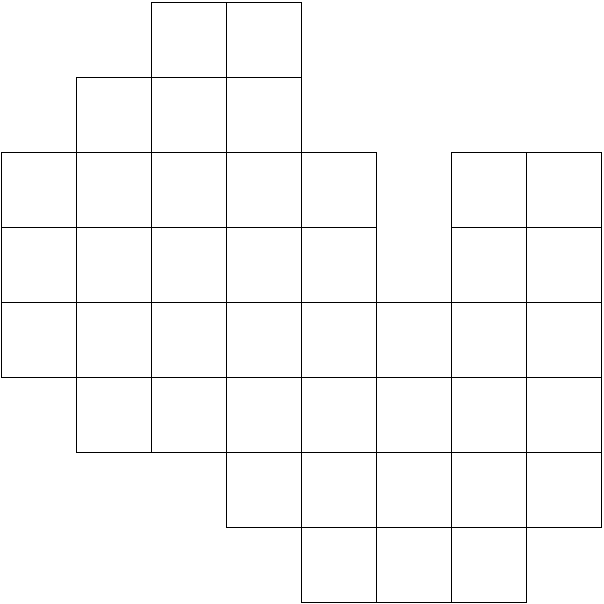
\includegraphics[height=2.5in]{../figures/domino}
\end{center}
\end{enumerate}
\end{quote}
%%%%%%%%%%%%%%%
\textbf{Solution: }
 Consider the bipartite graph $G$ with a vertex for each square
  and two squares are adjacent if they share an edge. This graph is
  bipartite since the squares can be colored black and white in a
  checkerboard pattern.

Any perfect tiling gives a perfect matching by simply selecting the
edges corresponding to the dominoes selected. And vice versa.

\begin{figure}[ht]
\begin{center}
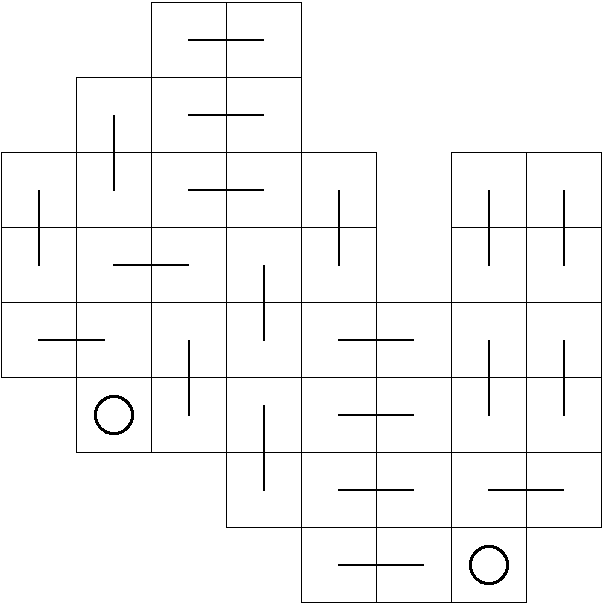
\includegraphics[height=2.3in]{../figures/domino2}
\end{center}
\caption{Maximum configuration of dominoes. \label{fig:domino2}}
\end{figure}

We claim that the configuration shown in Figure \ref{fig:domino2} is a
maximum one and so no perfect tiling exists. We will prove that the
matching $M$ corresponding to the configuration in Figure
\ref{fig:domino2} is maximum by showing that there is no augmenting
path as in the lecture. (Alternatively we could use Hall's theorem.)

Let $A$ be the set of black squares and $B$ the set of white squares.
Orient the edges of $G$ according to $M$, i.e. all the edges in $M$
are oriented from $B$ to $A$, and the edges not in $M$ are oriented
from $A$ to $B$ as in Figure \ref{fig:domino34}.

Let $v$ be the only exposed vertex of $A$ and $w$ be the only exposed
vertex of $B$, and consider $L$ to be the set of vertices reachable
from $v$ (the enclosed area in Figure \ref{fig:domino34}). Since $w$
is not in $L$ we obtain that no augmenting path exists.
\begin{figure}[ht]
\begin{minipage}[b]{0.5\linewidth} % A minipage that covers half the page
\begin{center}
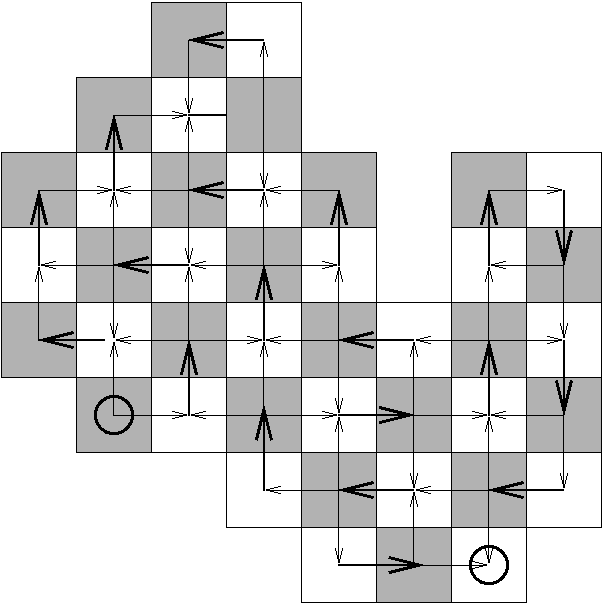
\includegraphics[height=2.3in]{../figures/domino3}
\end{center}
\caption{Oriented graph.}
\end{minipage}
\hspace{0.5cm} % To get a little bit of space between the figures
\begin{minipage}[b]{0.5\linewidth}
\begin{center}
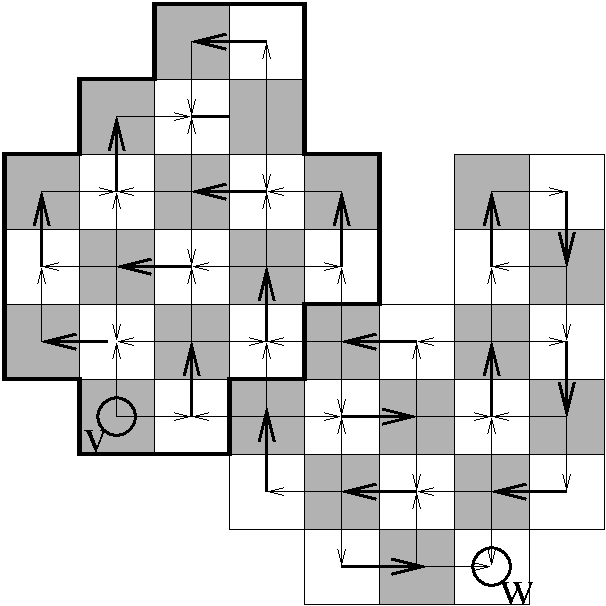
\includegraphics[height=2.3in]{../figures/domino4}
\end{center}
\caption{Set of reachable vertices from $v$.\label{fig:domino34}}
\end{minipage}
\end{figure}

We can also deduce the fact that no perfect matching exists from
Hall's theorem by observing that the 11 black vertices in $L$ (the
enclosed region on the right of Figure \ref{fig:domino34}) has only 10
(white) neighbors.


%%%%%%%%%%%%%%%%%%%%

\item[1-6]
\begin{quote}
Consider a bipartite graph $G=(V,E)$ with bipartition $(A,B)$: $V=A
\cup B$. Assume that, for some vertex sets $A_1\subseteq A$ and $B_1
\subseteq B$, there exists a matching $M_A$ covering all vertices in
$A_1$ and a matching $M_B$ covering all vertices in $B_1$. Prove that
there always exists a matching covering all vertices in $A_1\cup
B_1$.
\end{quote}

\textbf{Solution: }
Make a bipartite graph $H$ with edge set $M_A \cup M_B$ (and vertex set $V$). Then every vertex has $H$-degree at most $2$, and every vertex in $A_1 \cup B_1$ has $H$-degree at least $1$. So the connected components of $H$ consist of paths and (even) cycles, and every vertex of $A_1\cup B_1$ is contained in a nontrivial connected component of $H$. We will show that there is a matching $M$ of $H$ which covers all vertices of $A_1 \cup B_1$; since the edges of $H$ are a subset of the edges of $G$, this will solve the problem.

It's enough to show that every nontrivial connected component $P$ of $H$ has a matching $M_P$ which covers the vertices of $A_1\cup B_1$ which are contained in $P$. If $P$ is an even cycle or an odd path (with an even number of vertices), then $P$ has a perfect matching, and we take $M_P$ to be a perfect matching of $P$. If $P$ is an even path (with an odd number of vertices), then every matching of $P$ leaves some vertex of $P$ uncovered, so we must show that in this case at least one of the endpoints of $P$ is not contained in $A_1\cup B_1$. Note that since $P$ has length greater than $1$, no edge of $P$ can be in $M_A \cap M_B$, and the edges of $P$ alternate between edges of $M_A$ and $M_B$. Since $P$ has even length, the endpoints of $P$ are either both from $A$ or both from $B$, while exactly one of the first and last edges of $P$ is from $M_A$ and the other is from $M_B$. Thus, $P$ either has an endpoint in $A$ which is not covered by $M_A$ or an endpoint in $B$ which is not covered by $M_B$, and we can choose $M_P$ to be the matching of $P$ which covers all of $P$ other than this endpoint.

%%%%%%%%%%%%%%%%%%%%

\item[1-7] % from 2009
\begin{quote}
Consider a bipartite graph $G=(V,E)$ with bipartition $(A,B)$
($V=A\cup B$). Let ${\cal I}=\{X\subseteq A:$ there exists a matching
$M$ of $G$ such that all vertices of $X$ are matched$\}$.

Show that
\begin{enumerate}
\item
If $X\in {\cal I}$ and $Y\subseteq X$ then $Y\in {\cal I}$.
\item
If $X, Y\in {\cal I}$ and $|X|<|Y|$ then there exists $y\in Y\setminus
X$ such that $X\cup\{y\}\in {\cal I}$.
\end{enumerate}
(Later in the class, we will discuss matroids; properties (i) and
(ii) form the definition of independent sets of a matroid.)
\end{quote}
%%%%%%%%%%%%%%%
\textbf{Solution: }
\begin{enumerate}
\item Let $Y \subset X \in {\cal I}$. Since $X$ is an
independent set, there exists a matching $M_X$ that covers $X$. This
matching also covers $Y$. Hence $Y$ is an independent set.
\item Let $X,Y \in {\cal I}$ with $|X| < |Y|$. It follows that
there exist matchings $M_X$ and $M_Y$ such that $M_X$ covers $X$ and
$M_Y$ covers $Y$. Consider the graph $G' = (V,M_X \Delta M_Y)$. The
set of edges of $G'$ is the union of paths and cycles.

If $M_X$ covers some element $y$ in $Y\setminus X$. Then $X+ y$ is an
independent set.

Otherwise, all the vertices in $Y\setminus X$ are of degree 1 in
$G'$. Since $|Y| > |X|$, we have $|Y\setminus X| > |X\setminus
Y|$. Therefore, by the previous observation, there are more degree 1
vertices in $Y\setminus X$ than in $X \setminus Y$. It follows that
there exists a path $P$ in the decomposition of $G'$ starting in a
vertex $y \in Y\setminus X$ and not ending in $X$. We conclude that
$M_X \Delta P$ is a matching of $G$ that covers $X \cup \{y\}$. Thus,
$X + y$ is an independent set.
\end{enumerate}


\item[1-10] % revised by Cesar Cuenca
\begin{quote}
Consider a bipartite graph $G=(V,E)$ with bipartition $(A,B)$. For
$X\subseteq A$, define $\operatorname{def}(X)=|X|-|N(X)|$ where $N(X)=\{b\in B:
\exists a\in X$ with $(a,b)\in E\}$. Let $$\operatorname{def}_{max}=
\max_{X\subseteq A} \operatorname{def}(X).$$ Since $\operatorname{def}(\emptyset)=0$, we have
$\operatorname{def}_{max}\geq 0$.
\begin{enumerate}
\item
Generalize Hall's theorem by showing that the maximum size of a
matching in a bipartite graph $G$ equals $|A|-\operatorname{def}_{max}$.
\item
For any 2 subsets $X, Y\subseteq A$, show that
$$\operatorname{def}(X\cup Y) + \operatorname{def}(X\cap Y) \geq \operatorname{def}(X) + \operatorname{def}(Y).$$
\item (Optional:) Consider a 0-1 matrix. How are the following things related? 1. The maximal number of rooks (as in chess) that can be placed on a 1 in the matrix without attacking one another. 2. The minimal number of vertical or horizontal lines that contain all the 1's in the matrix. 3. The $a\times b$ all-zero submatrix with $a + b$ largest.
\end{enumerate}
\end{quote}


\begin{enumerate}
\item
Clearly, the size of a maximum matching cannot be more than
$|A|-\operatorname{def}_{max}$ (since any matching has at
most $|A|-|X|$ edges incident to $A-X$ and at most $|N(X)|$ edges
incident to $X$).

Conversely, consider the minimum vertex cover $C$ and let
$X=A\setminus C$. Observe that $N(X)\subseteq C\cap B$, and thus
$$\operatorname{def}(X) =|X|-|N(X)|\geq |A\setminus C| - |C \cap B| =
|A| - |C \cap A|- |C\cap B|=|A|-|C|.$$  Therefore
$\operatorname{def}_{max}\geq |A|-|C|$ and the result follows from
K\"onig's theorem.
\item
This is a simple counting argument. First of all, $$|X\cup Y|+|X\cap
Y|=|X|+|Y|.$$ Furthermore, $$|N(X\cup Y)| + |N(X\cap Y)| \leq |N(X)| +
|N(Y)|,$$ since every vertex $b$ in $B$ contributes at least as much
to the right-hand-side than to the left-hand-side. Indeed, if $b\in
N(X\cup Y)\setminus N(X\cap Y)$, it should be either in $N(X)$ or in
$N(Y)$, while if $b\in N(X \cap Y)$, it should be in both $N(X)$ and in $N(Y)$.

\item Associate a bipartite graph (with bipartition $(A,B)$) to a given 0-1 matrix (of size, say, $n\times m$) as follows: its vertices are the rows ($A$) and columns ($B$), and an edge between a row and a column is drawn if the corresponding matrix entry is 1. Under this correspondence, we have the following dictionary.
    \begin{itemize}
      \item Placing rooks on 1s (without attacking one another) $\longleftrightarrow$ a matching in the graph.
      \item Vertical or horizontal lines that contain all the 1's in the matrix $\longleftrightarrow$ a vertex cover in the graph.
      \item An $a\times b$ all-zero submatrix $\longleftrightarrow$ sets $A' \subset A, |A'|=a$, $B' \subset B, |B'|=b$ such that $N(A') \cap B' = \emptyset$.
    \end{itemize}
    With that in mind, we can relate those three numbers as follows. Let $x_1$ be the maximal number of rooks placed on 1s, $x_2$ be the minimal number of lines that contain all the 1's, and $x_3$ be the largest $a+b$ such that there is an $a\times b$ all-zero submatrix. For $x_3$, it is convenient to assume that degenerate $0\times m$ matrices are allowed, so $x_3 \ge m$. Then by K\H{o}nig's theorem, $x_1 = x_2$; and by extended Hall's theorem, $x_3 = n+m - x_1$.
\end{enumerate}

%%%%%

\iffalse
\item[1-15]
\begin{quote}
Consider a bipartite graph $G=(V,E)$ in which every vertex has degree
$k$ (a so-called $k$-regular bipartite graph). Prove that such a graph
always has a perfect matching in two different ways:
\begin{enumerate}
\item
by using K\"onig's theorem,
\item
by using the linear programming formulation we have derived in this
section.
\end{enumerate}
\end{quote}
%%%%%%%%%%%%%%%

\textbf{Solution: }
Let $A$, $B$ be the bipartition of $V$.
\begin{enumerate}
  \item  Because of
  $k$-regularity, we have $|A| = |B|$. Let $n = |A|$.
  By K\"{o}nig's theorem, let $C$ be a minimum vertex cover of
  size equal to the maximum matching. Then, $N(A \setminus C)
  \subseteq B \cap C$, and because of $k$-regularity, $|A  \setminus C| \leq |B \cap C|$ (count the number of edges incident to vertices in $A\setminus C$ in two ways). Similarly, $|B
  \setminus C| \leq |A \cap C|$. Adding the inequalities we get $|V \setminus C|
  \leq |C|$, which implies that $|C| \geq |V|/2$.

  \item Any integer solution of the LP formulation
    \lps
  &  &  & \mbox{Min} &  \sum_{i,j} c_{ij} x_{ij} \\
  & \lefteqn{\mbox{subject to:}} \\
  &        &   &  &   \sum_j x_{ij} =1 & i\in A \\
  &        &   &  &   \sum_i x_{ij} =1 & j\in B \\
  &        &   &  &  x_{ij}\geq 0 & i\in A, j\in B
\elps  is a perfect  matching. Also, all the extreme points (if any) of the LP are integral (see
  lecture notes on bipartite matching).
  Thus, it is enough to prove that the LP is feasible (so it will have
  at least one extreme point), and this is indeed the case as $x_{ij}=
  1/k$ for all edges $(i,j)$ is a feasible solution.
\end{enumerate}
(One needs to add some assumption for the result to be true for non-bipartite graphs; indeed a cycle on 3 vertices does not have a perfect matching.)
\fi

%%%%%%%%%%%%%%%%%

\item[1-18]

\begin{quote}
We have shown that there always exists a solution $x$ to the linear program (P) with all components integral. Reprove this result in the following way.

Take a (possibly non-integral) optimum solution $x^*$. If there are many optimum solutions, take one with as few non-integral values $x^*_{ij}$ as possible. Show that, if $x^*$ is not integral, there exists a cycle $C$ with all edges $e = (i, j) \in C$ having a non-integral value $x^*_{ij}$. Now show how to derive another optimum solution with fewer non-integral values, leading to a contradiction.

(Optional:) Conclude that the doubly stochastic matrices (the set of $n\times n$ nonnegative matrices with unit row and column sums) are the convex hull of the permutation matrices (the matrices with exactly $n$ ones, no two in the same row or column).
\end{quote}

Let us first recall the linear program (P):
    \lps
  &  &  & \mbox{Min} &  \sum_{i,j} c_{ij} x_{ij} \\
  & \lefteqn{\mbox{subject to:}} \\
  &        &   &  &   \sum_j x_{ij} =1 & i\in A \\
  &        &   &  &   \sum_i x_{ij} =1 & j\in B \\
  &        &   &  &  x_{ij}\geq 0 & i\in A, j\in B
\elps

Let $x^*$ be an optimum solution of (P) with the fewest non-integral values $x^*_{ij}$. We may assume that there exists at least one $ij$ with non-integral $x^*_{ij}$ (otherwise, we are done). Let $G = (V, E)$ be the bipartite graph with bipartition $(A, B)$ ($V = A \cup B$) and the edge set
$$
E = \{ (i, j)\in A \times B: x^*_{ij} \text{ is not integral}\}.
$$
We claim that for every $i \in V$ the degree of $i$ with respect to $G$ is not equal to one. Suppose not. Then there is $i \in A$ and $j' \in B$ (or change the role of $A$ and $B$) such that $x^*_{ij'}$ is non-integral, and $x^*_{ij}$ is integral for all $j \in B \setminus \{j'\}$. Since $\sum_{j\in B} x^*_{ij} = 1$, we have
$$
x^*_{ij'} = 1- \sum_{j \in B \setminus \{j'\}} x^*_{ij}.
$$
This is a contradiction because the left-hand side is non-integral but the right-hand side is integral.

Now, note that every connected component of $G$ is either an isolated vertex or a graph in which all vertices have degree at least 2. Moreover, there exists a connected component of the latter type because $G$ has at least one edge. This implies that there exists a cycle $C$ in $G$.

Let us construct an optimum solution $x'$ with fewer non-integral values than $x^*$. Let $e_1,e_2,\dotsc,e_\ell$ be edges of $C$ in cyclic order. Since $G$ is bipartite, the length $\ell$ of $C$ must be an even number. Let
$$
x'_{ij} = \begin{cases}
x_{ij}^* - t & \text{ if $ij = e_{k}$ for some odd $k$} \\
x_{ij}^* + t & \text{ if $ij = e_{k}$ for some even $k$} \\
x_{ij}^* & \text{ otherwise.}
\end{cases}
$$
Note that $x'$ is a feasible solution as long as every entry of $x'$ is positive, i.e.
$$
-\min_{\text{odd } k} x_{e_{k}}^* \leq t \leq \min_{\text{even }k} x_{e_{k}}^*
$$
Moreover, the objective function has the value
$$
\sum_{ij} c_{ij} x'_{ij} = \sum_{ij} c_{ij} x^*_{ij} + t \sum_{k=1}^{\ell} (-1)^k c_{e_k}.
$$
Since $x^*$ is an optimum solution, we must have
$$
\sum_{k=1}^t (-1)^k c_{e_k} = 0
$$
because otherwise we can set $t$ to be a value such that the objective value of $x'$ is smaller than that of $x^*$. This implies that $x'_{ij}$ is another optimum solution as long as it is feasible.

Set $t$ to be $\min_{\text{even $k$}} x_{e_k}^*$. Let $k'$ be an index such that $t = x_{e_{k'}}^*$. Then, $x'_{e_{k'}} = 0$ so $x'$ has fewer non-integral values than $x^*$ which contradicts the minimality of $x^*$.

For the optional part, we notice that the feasible solutions of program (P) constitute exactly the set of doubly stochastic matrices. We need to conclude that it is the same as the convex hull of the permutation matrices. This follows from the following standard facts from convexity.
\begin{itemize}
  \item Every bounded polyhedron can be equivalently described as the convex hull of its \emph{extreme points}, or \emph{vertices}, that is, points that are in the set, and that do not belong to the relative interior of any straight line interval in the set. This is properly explained later in the course.
  \item Every extreme point can be obtained as an optimal solution in (P) for some linear functional $\sum c_{ij} x_{ij}$. This can be seen by taking coefficients $c_{ij}$ such that the face of $P$ corresponding to this direction contains that extreme point. 
\end{itemize}

%%
\item[1-11] % from Chiheon?
\begin{quote}
Let $S=\{1,2, \cdots, n\}$. Let $A_k$ be the set of all subsets of $S$ of cardinality $k$ (thus $|A_k|={n \choose k}$). Let $k<\frac{n}{2}$. Consider the graph $G_k$ with bipartition $A_k$ and $A_{k+1}$, and with $E=\{(a,b) | a\in A_k, b\in A_{k+1}$ and $a\subset b\}$.
\begin{enumerate}
\item
Prove that the maximum matching in $G_k$ has size $A_k$ (remember $k<n/2$).
\item
Prove {\it Sperner's lemma}. The maximum number of subsets of $S$ such that no subset is contained into another is ${n \choose {\lfloor n/2 \rfloor}}$.
\end{enumerate}
\end{quote}
%%%%%%%%%%%

\begin{enumerate}
\item Let $X$ be a subset of $A_k$. Note that any vertex in $A_k$ has degree $n-k$ in $G_k$. So, the number of edges between $X$ and $N(X)$ is $(n-k)|X|$. On the other hand, the number of edges adjacent to $N(X)$ is $(k+1)|N(X)|$ since any vertex in $A_{k+1}$ has degree $k+1$. Thus, $(n-k)|X| \leq (k+1)|N(X)|$. Since $k < \frac{n}{2}$, we have
$$
|X| \leq \frac{k+1}{n-k}|N(X)| \leq |N(X)|.
$$
By Hall's Theorem, there is a matching in $G_k$ covering $A_k$.

\item For a collection $\mathcal{C}$ of subsets of $S$, we call it a {\it chain} if for any $x, y \in \mathcal{C}$ either $x \subset y$ or $y \subset x$. In other words, chain is a sequence of subsets $a_1 \subset a_2 \subset \dotsc \subset a_k$. On the other hand, we call a collection $\mathcal{F}$ of subsets of $S$ an {\it antichain}, if no subset is contained in another. Note that any chain and antichain can share at most one element.

We claim that the collection of all subsets of $S$ can be partitioned into $\binom{n}{\lceil n/2 \rceil}$ chains. This implies that the size of antichain is at most $\binom{n}{\lceil n/2 \rceil}$, since an antichain can have at most one element from each chain.

Recall part (a). We know that $G_k$ has a matching covering $A_k$ if $k < \lceil \frac{n}{2} \rceil$. Similarly, if $k \geq \lceil \frac{n}{2} \rceil$ then $G_k$ has a matching covering $A_{k+1}$. Let $M$ be the union of those matchings in $G_k$ for $k=0,1,\dotsc,n-1$. Note that $M$ consists of disjoint paths, and for each path there are indices $k$ and $\ell$ such that the path is of the form $a_k a_{k+1} \dotsc a_\ell$ where $a_j \in A_j$ for $j=k, \dotsc, \ell$ and $a_j a_{j+1} \in M$. Moreover, each path contains exactly one element from $A_{\lceil \frac{n}{2} \rceil}$. Since each path is a chain, we have $\binom{n}{\lceil n/2 \rceil}$ disjoint chains covering all subsets of $S$.
\end{enumerate}

%%%%%%%%%%%%%%%

\item[1-20]
\begin{quote}
  For the assignment problem, the greedy algorithm (which repeatedly
  finds the minimum cost edge disjoint from all the previously
  selected edges) can lead to a solution whose cost divided by the
  optimum cost can be arbitrarily large (even for graphs with 2
  vertices on each side of the bipartition).

Suppose now that the cost comes from a  metric, even just a line
metric. More precisely, suppose that the bipartition is $A \cup B$
with $|A|=|B|=n$ and the $i$th vertex of $A$ (resp. the $j$th vertex
of $B$) is associated with $a_i\in \R$ (resp. $b_j\in B$). Suppose
that the cost between these vertices is given by $c_{ij}=|a_i-b_j|$.

Consider the greedy algorithm: select the closest pair of vertices,
one from $A$ and from $B$, match them together, delete them, and
repeat until all vertices are matched. For these line metric
instances, is the cost of the greedy solution always upper bounded by
a constant (independent of $n$) times the optimum cost of the
assignment? If so, prove it; if not, give a family of examples
(parametrized by $n$) such that the corresponding ratio becomes
arbitrarily large.
\end{quote}

We will give a family of examples (based on the Cantor set) where the ratio between the cost of the greedy solution and the cost of the optimum assignment becomes arbitrarily large. Our $k$th example will have $n = 2^k$ vertices in $A$ and in $B$, and cost ratio slightly smaller than $2\cdot (\frac{3}{2})^k - 1$.

Fix some small $\epsilon > 0$. We define sets $A_k, B_k \subseteq \mathbb{R}$ inductively, as follows. For $k = 0$, we set $A_0 = \{0\}$ and $B_0 = \{1+\epsilon\}$. For $k \ge 1$, we let
\[
A_k = A_{k-1} \cup ((\max(B_{k-1}) + 3^{k-1}) + A_{k-1})
\]
and
\[
B_k = B_{k-1} \cup ((\max(B_{k-1}) + 3^{k-1}) + B_{k-1}) = (1+\epsilon) + A_k.
\]
For example, we have
\[
A_1 = \{0, 2+\epsilon\}, \;\;\;\;\; B_1 = \{1+\epsilon, 3+2\epsilon\}
\]
and
\[
A_2 = \{0, 2+\epsilon, 6+2\epsilon, 8+3\epsilon\}, \;\;\;\;\; B_2 = \{1+\epsilon, 3+2\epsilon, 7+3\epsilon, 9+4\epsilon\}.
\]
Let $a_0, ..., a_{2^k-1}$ be the elements of $A_k$, in sorted order, and define $b_0, ..., b_{2_k-1}$ similarly. Inducting on $k$, it's easy to see that the greedy algorithm assigns each $a_i$ to $b_{i-1}$ for $0 < i < 2^k$, and assigns $a_0$ to $b_{2^k-1}$, with total cost $3^k - 2^k + (3^k + 2^k\epsilon)$.

On the other hand, the optimal assignment is at least as good as what we get by assigning each $a_i$ to $b_i$, which has total cost $2^k\cdot(1+\epsilon)$. This gives a cost ratio of
\[
\frac{2\cdot 3^k - 2^k + 2^k\epsilon}{2^k + 2^k\epsilon},
\]
and this goes to infinity as $k$ gets large.


\end{enumerate}
\end{document}

